%
% firmware.tex
%
% Copyright The EPS 2.0 Contributors.
%
% EPS 2.0 Documentation
%
% This work is licensed under the Creative Commons Attribution-ShareAlike 4.0
% International License. To view a copy of this license,
% visit http://creativecommons.org/licenses/by-sa/4.0/.
%

%
% \brief Firmware project chapter.
%
% \author Gabriel Mariano Marcelino <gabriel.mm8@gmail.com>
% \author Yan castro de Azeredo <yan.ufsceel@gmail.com>
%
% \version 0.3.0
%
% \date 2021/03/07
%

\chapter{Firmware} \label{ch:firmware}

\section{Product tree}

The product tree of the firmware part of the EPS 2.0 module is available in \autoref{fig:product-tree-fw}.

\begin{figure}[!ht]
    \begin{center}
        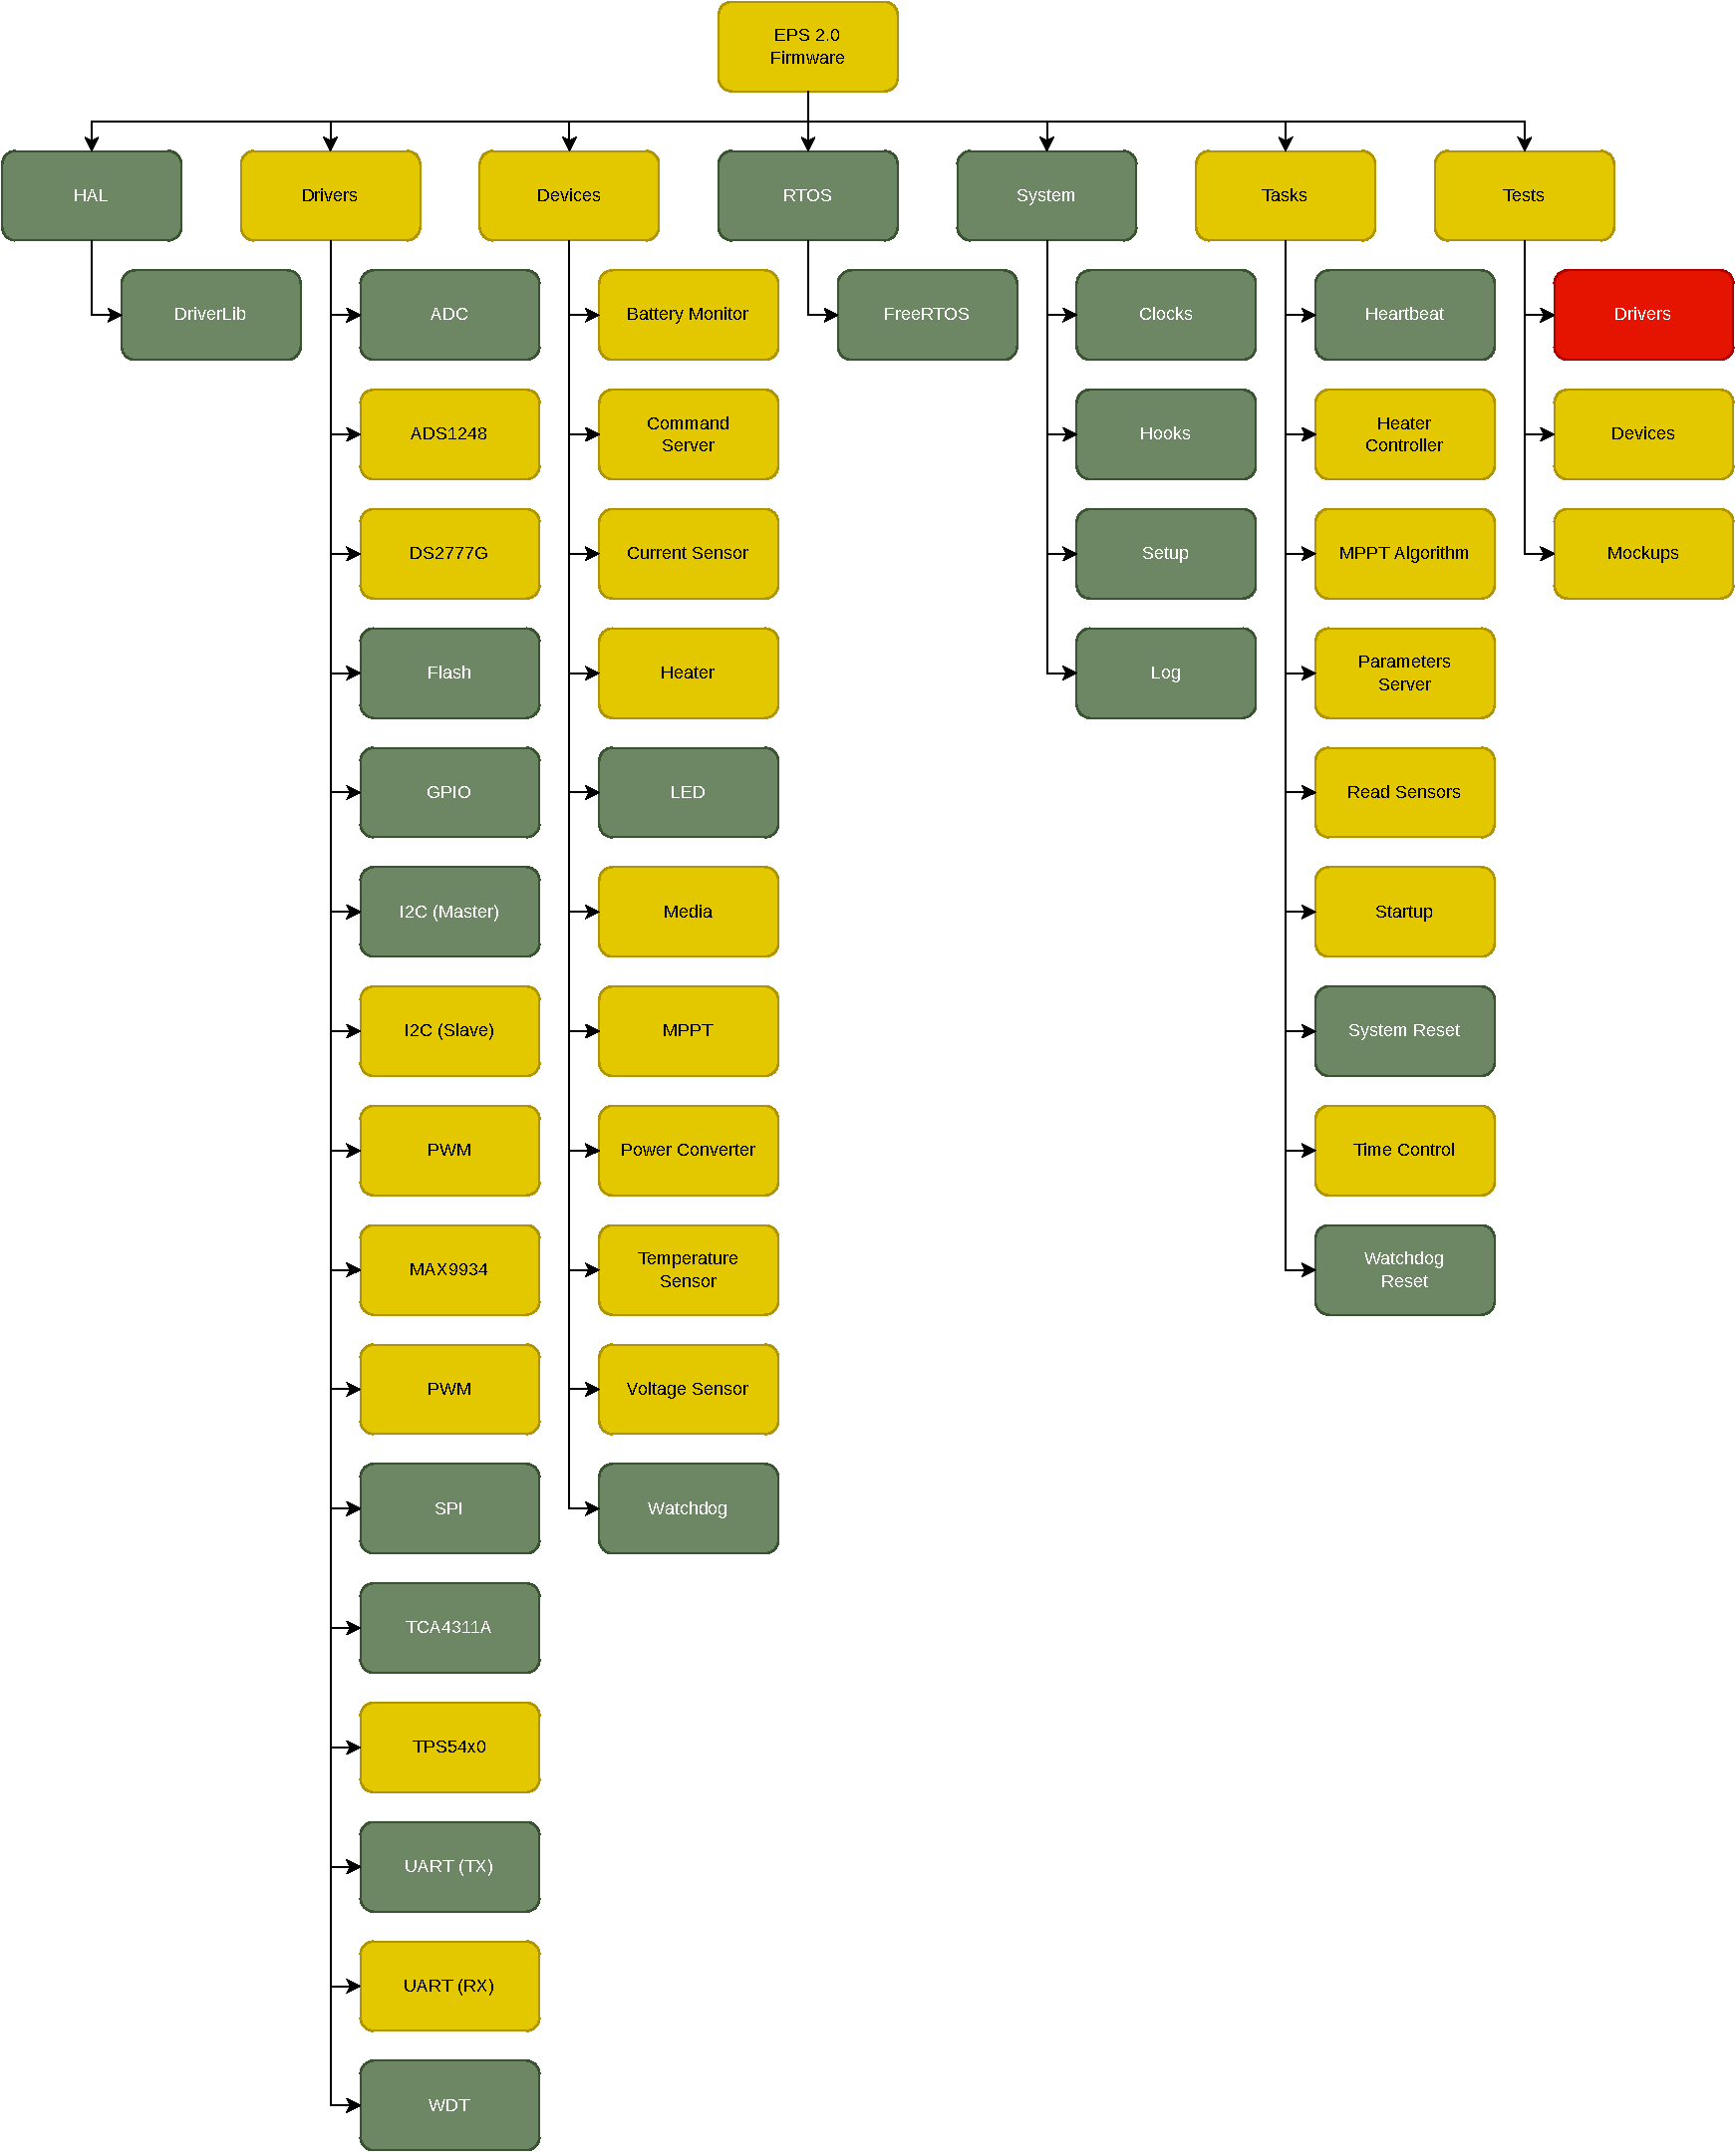
\includegraphics[width=\textwidth]{figures/product-tree-fw.pdf}
        \caption{Product tree of the firmware of the EPS 2.0 module.}
        \label{fig:product-tree-fw}
    \end{center}
\end{figure}

\section{Dependencies}

\section{Tasks}

A list of the firmware tasks can be seen in the \autoref{tab:firmware-tasks}.

\begin{table}[!h]
    \centering
    \begin{tabular}{lccccc}
        \toprule[1.5pt]
        \textbf{Name}          & \textbf{Priority} & \textbf{Initial delay [ms]} & \textbf{Period [ms]} & \textbf{Stack [bytes]} \\
        \midrule
        Startup (boot)         & Highest           & 0                           & Aperiodic            & 500                    \\
        Watchdog reset         & Lowest            & 0                           & 100                  & 128                    \\
        Heartbeat              & Lowest            & 0                           & 500                  & 128                    \\
        System reset           & High              & 0                           & 36000000             & 128                    \\
        Battery Heater Control & TBD               & 0                           & TBD                  & TBD                    \\
        Read sensors           & Medium            & 0                           & 60000                & 128                    \\
        CSP Server             & Lowest            & 0                           & 500                  & 1024                   \\
        MPPT                   & TBD               & TBD                         & TBD                  & TBD                    \\
        Beacon package         & TBD               & TBD                         & TBD                  & TBD                    \\
        OBDH package           & Highest           & 4500   & Called by ISR\nomenclature{\textbf{ISR}}{\textit{Interrupt Service Routine.}}   & TBD \\
        \bottomrule[1.5pt]
    \end{tabular}
    \caption{Firmware tasks.}
    \label{tab:firmware-tasks}
\end{table}

\subsection{Startup (boot)}

\subsection{Watchdog reset}

\subsection{Heartbeat}

\subsection{System reset}

\subsection{Battery heater control}

\subsection{Read sensors}

\subsection{MPPT}

\subsection{Beacon package}

\subsection{OBDH package}

\section{Variables and Parameters}

A list of all the variables of EPS with their identification number (ID) and variable type that can be read from the sensors and peripherals is seen in the \autoref{tab:eps2-variables}.

\begin{longtable}[c]{cL{0.72\textwidth}lc}
    \toprule[1.5pt]
    \textbf{ID} & \textbf{Name/Description} & \textbf{Type} & \textbf{Access} \\
    \midrule
    0   & Time counter in millseconds                                       & uint32 & R \\
    1   & Temperature of the $\mu$C in K                                    & uint16 & R \\
    2   & EPS circuitry current in mA                                       & uint16 & R \\
    \multirow{18}{*}{3} & Last reset cause: & \multirow{18}{*}{uint8} & \multirow{18}{*}{R} \\
        & - 0x00 = No interrupt pending                                     &        &  \\
        & - 0x02 = Brownout (BOR)                                           &        &  \\
        & - 0x04 = RST/NMI (BOR)                                            &        &  \\
        & - 0x06 = PMMSWBOR (BOR)                                           &        &  \\
        & - 0x08 = Wakeup from LPMx.5 (BOR)                                 &        &  \\
        & - 0x0A = Security violation (BOR)                                 &        &  \\
        & - 0x0C = SVSL (POR)                                               &        &  \\
        & - 0x0E = SVSH (POR)                                               &        &  \\
        & - 0x10 = SVML\_OVP (POR)                                          &        &  \\
        & - 0x12 = SVMH\_OVP (POR)                                          &        &  \\
        & - 0x14 = PMMSWPOR (POR)                                           &        &  \\
        & - 0x16 = WDT time out (PUC)                                       &        &  \\
        & - 0x18 = WDT password violation (PUC)                             &        &  \\
        & - 0x1A = Flash password violation (PUC)                           &        &  \\
        & - 0x1C = Reserved                                                 &        &  \\
        & - 0x1E = PERF peripheral/configuration area fetch (PUC)           &        &  \\
        & - 0x20 = PMM password violation (PUC)                             &        &  \\
        & - 0x22 to 0x3E = Reserved                                         &        &  \\
    4   & Reset counter                                                     & uint16 & R \\
    5   & -Y and +X sides solar panel voltage in mV                         & uint16 & R \\
    6   & -X and +Z sides solar panel voltage in mV                         & uint16 & R \\
    7   & -Z and +Y sides solar panel voltage in mV                         & uint16 & R \\
    8   & -Y side solar panel current in mA                                 & uint16 & R \\
    9   & +Y side solar panel current in mA                                 & uint16 & R \\
    10  & -X side solar panel current in mA                                 & uint16 & R \\
    11  & +X side solar panel current in mA                                 & uint16 & R \\
    12  & -Z side solar panel current in mA                                 & uint16 & R \\
    13  & +Z side solar panel current in mA                                 & uint16 & R \\
    14  & MPPT 1 duty cycle in \% (writable just in manual mode)            & uint8  & R/W \\
    15  & MPPT 2 duty cycle in \% (writable just in manual mode)            & uint8  & R/W \\
    16  & MPPT 3 duty cycle in \% (writable just in manual mode)            & uint8  & R/W \\
    17  & Total solar panels output voltage after MPPT in mV                & uint16 & R \\
    18  & Main power bus voltage in mV                                      & uint16 & R \\
    19  & RTD0 temperature in K                                             & uint16 & R \\
    20  & RTD1 temperature in K                                             & uint16 & R \\
    21  & RTD2 temperature in K                                             & uint16 & R \\
    22  & RTD3 temperature in K                                             & uint16 & R \\
    23  & RTD4 temperature in K                                             & uint16 & R \\
    24  & RTD5 temperature in K                                             & uint16 & R \\
    25  & RTD6 temperature in K                                             & uint16 & R \\
    26  & Batteries voltage in mV                                           & uint16 & R \\
    27  & Batteries current in mA                                           & uint16 & R \\
    28  & Batteries average current in mA                                   & uint16 & R \\
    29  & Batteries accumulated current in mA                               & uint16 & R \\
    30  & Batteries charge in mAh                                           & uint16 & R \\
    31  & Battery monitor IC temperature in K                               & uint16 & R \\
    32  & Battery monitor status register                                   & uint8  & R \\
    33  & Battery monitor protection register                               & uint8  & R \\
    34  & Battery monitor cycle counter                                     & uint8  & R \\
    35  & Battery monitor Remaining Active-Absolute Capacity (RAAC) in mAh  & uint16 & R \\
    36  & Battery monitor Remaining Standby-Absolute Capacity (RSAC) in mAh & uint16 & R \\
    37  & Battery monitor Remaining Active-Relative Capacity (RARC) in \%   & uint8  & R \\
    38  & Battery monitor Remaining Standby-Relative Capacity (RSRC) in \%  & uint8  & R \\
    39  & Battery heater 1 duty cycle in \% (writable just in manual mode)  & uint8  & R/W \\
    40  & Battery heater 2 duty cycle in \% (writable just in manual mode)  & uint8  & R/W \\
    41  & Hardware version                                                  & uint8  & R \\
    42  & Firmware version (ex.: ``v1.2.3''' = 0x00010203)                  & uint32 & R \\
    43  & MPPT 1 mode (0x00 = automatic, 0x01 = manual)                     & uint8  & R/W \\
    44  & MPPT 2 mode (0x00 = automatic, 0x01 = manual)                     & uint8  & R/W \\
    45  & MPPT 3 mode (0x00 = automatic, 0x01 = manual)                     & uint8  & R/W \\
    46  & Battery heater 1 mode (0x00 = automatic, 0x01 = manual)           & uint8  & R/W \\
    47  & Battery heater 2 mode (0x00 = automatic, 0x01 = manual)           & uint8  & R/W \\
    48  & Device ID (0xEEE2)                                                & uint16 & R \\
    \bottomrule[1.5pt]
    \caption{Variables and parameters of the EPS 2.0.}
    \label{tab:eps2-variables}
\end{longtable}

\section{Operating System}

As operating system the FreeRTOS 10 \cite{freertos} is being used. FreeRTOS is a market-leading real-time operating system (RTOS) for microcontrollers and small microprocessors. Distributed freely under the MIT open source license, FreeRTOS includes a kernel and a growing set of IoT libraries suitable for use across all industry sectors. FreeRTOS is built with an emphasis on reliability and ease of use.

The main configuration parameters of the operating system in this project are availabe in \autoref{tab:freertos-config}.

\begin{table}[!h]
    \centering
    \begin{tabular}{lrr}
        \toprule[1.5pt]
        \textbf{Parameter}       & \textbf{Value} & \textbf{Unit} \\
        \midrule
        Version                  & v10.2.0        & - \\
        Tick rate (Hz)           & 1000           & Hz \\
        CPU clock (HZ)           & 32             & MHz \\
        Max. priorities          & TBD            & - \\
        Heap size                & TBD            & bytes \\
        Max. length of task name & 20             & - \\
        \bottomrule[1.5pt]
    \end{tabular}
    \caption{FreeRTOS main configuration parameters.}
    \label{tab:freertos-config}
\end{table}

More details of the used configuration parameters can be seen in the file \textit{\href{https://github.com/spacelab-ufsc/eps2/blob/master/firmware/config/FreeRTOSConfig.h}{firmware/config/FreeRTOSConfig.h}} from \cite{eps2}.

\section{Hardware Abstraction Layer (HAL)}

As the Hardware Abstraction Layer (HAL\nomenclature{\textbf{HAL}}{\textit{Hardware Abstraction Layer.}}), the DriverLib \cite{driverlib} from Texas Instruments is begin used. It is the official API to access the registers of the MSP430 microcontrollers.

The DriverLib is meant to provide a ``software'' layer to the programmer in order to facilitate higher level of programming compared to direct register accesses. By using the high level software APIs provided by DriverLib, users can create powerful and intuitive code which is highly portable between not only devices within the MSP430 platform, but between different families in the MSP430/MSP432 platforms.
